\documentclass[tikz,border=9pt]{standalone}
\usepackage[utf8]{inputenc}
\usepackage[OT4,plmath]{polski}
\usepackage{amsmath}
\begin{document}
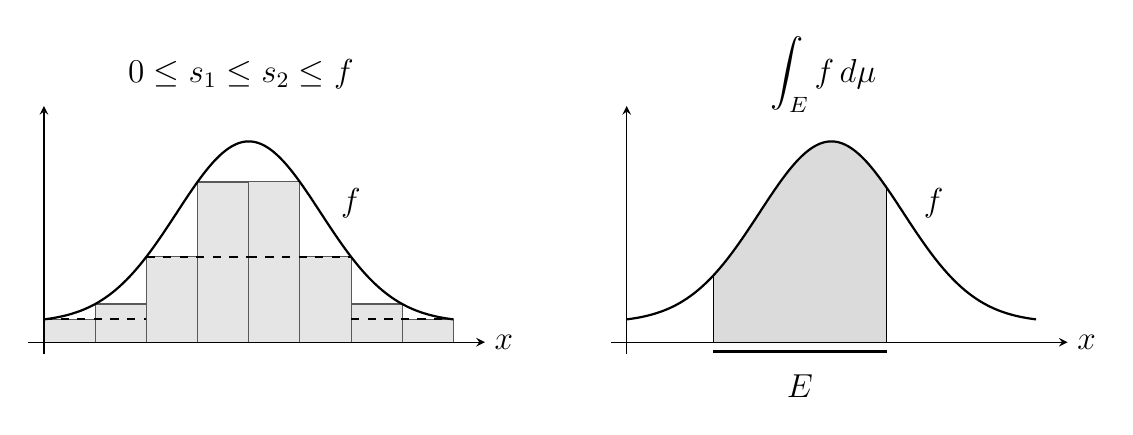
\begin{tikzpicture}[font=\large,>=stealth]
  \begin{scope}
    \node at (2.5,3.4) {$0\leq s_1\leq s_2\leq f$};
    \foreach \i in {0,...,7} {
      \pgfmathsetmacro{\lft}{0.65*\i}
      \pgfmathsetmacro{\rgt}{\lft+0.65}
      \pgfmathsetmacro{\htval}{min(0.25+2.3*exp(-0.6*(\lft-2.6)^2),0.25+2.3*exp(-0.6*(\rgt-2.6)^2))}
      \filldraw[fill=black!10,draw=black!65] (\lft,0) rectangle (\rgt,\htval);
    }
    \foreach \i in {0,...,3} {
      \pgfmathsetmacro{\lft}{1.3*\i}
      \pgfmathsetmacro{\rgt}{\lft+1.3}
      \pgfmathsetmacro{\htval}{min(0.25+2.3*exp(-0.6*(\lft-2.6)^2),0.25+2.3*exp(-0.6*(\rgt-2.6)^2))}
      \draw[thick,dashed] (\lft,\htval)--(\rgt,\htval);
    }
    \draw[thick,domain=0:5.2,samples=90,smooth]
      plot (\x,{0.25+2.3*exp(-0.6*(\x-2.6)^2)});
    \node[above right] at (3.65,1.45) {$f$};
    \draw[->] (-0.2,0)--(5.6,0) node[right] {$x$};
    \draw[->] (0,-0.15)--(0,3.0);
  \end{scope}
  \begin{scope}[xshift=7.4cm]
    \node at (2.5,3.4) {$\displaystyle\int_E f\,d\mu$};
    \fill[black!14] (1.1,0)--plot[domain=1.1:3.3,samples=50]
      (\x,{0.25+2.3*exp(-0.6*(\x-2.6)^2)})--(3.3,0)--cycle;
    \draw[thick,domain=0:5.2,samples=90,smooth]
      plot (\x,{0.25+2.3*exp(-0.6*(\x-2.6)^2)});
    \draw (1.1,0)--(1.1,{0.25+2.3*exp(-0.6*(1.1-2.6)^2)});
    \draw (3.3,0)--(3.3,{0.25+2.3*exp(-0.6*(3.3-2.6)^2)});
    \draw[->] (-0.2,0)--(5.6,0) node[right] {$x$};
    \draw[->] (0,-0.15)--(0,3.0);
    \draw[very thick] (1.1,-0.12)--(3.3,-0.12);
    \node[below=5pt] at (2.2,-0.12) {$E$};
    \node[above right] at (3.65,1.45) {$f$};
  \end{scope}
\end{tikzpicture}
\end{document}
